\section{Soft Actor-Critic Grundlagen}
\subsection{Grundlegender Aufbau}
\begin{frame}{Einordnung}
	\begin{itemize}
		\item Soft Actor-Critic ist ein off-policy Algorithmus mit Ähnlichkeiten zu DDPG und TD3  
		\item Im Gegensatz zu diesen nutzt Soft Actor-Critic jedoch eine stochastische Policy
		\item Durch den off-policy Ansatz besitzt Soft Actor-Critic eine hohe Probeneffizienz 
		\item Die Stabilität kann im Vergleich zu DDPG und TD3 erhöht werden 
	\end{itemize} 
\end{frame}


\begin{frame}{Actor-Critic}
	\begin{itemize}
		\item Soft Actor Critic nutzt einen Actor-Critic Ansatz
		\item Actor lernt eine Policy
		\item Critic lernt eine Value Function
	\end{itemize} 
	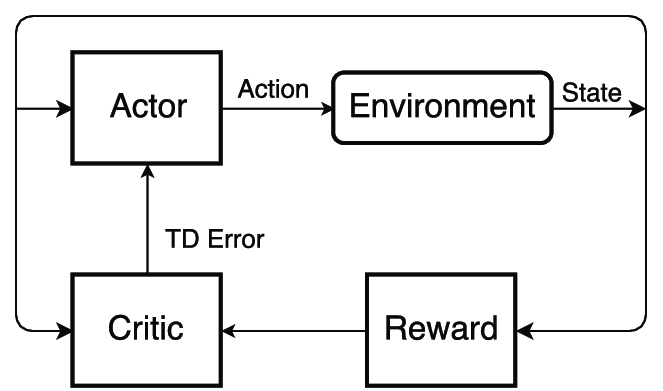
\includegraphics[width=190pt]{figures/A-regular-actor-critic-model-TD-temporal-difference.png}
\end{frame}

\begin{frame}{Maximierung der Entropie}
	\begin{itemize}
		\item Standard Reinforcment Lerning maximiert die Belohnung
		\begin{equation}
			\sum_{t=0}^T \mathbb{E}_{(s_t,a_t)\sim\rho_\pi}[{\mathnormal{r}(s_t,a_t)}] \notag
		\end{equation}
		\item Soft Actor-Critic maximiert zusätzlich noch die Entropie
		\begin{equation}
			\sum_{t=0}^T \mathbb{E}_{(s_t,a_t)\sim\rho_\pi}[{\mathnormal{r}(s_t,a_t)} + \alpha \mathcal{H}(\pi(\cdot|s_t))] \notag
		\end{equation}
	\end{itemize} 
\end{frame}

\begin{frame}{Entropie}
	\begin{itemize}
		
		\item Durch die Maximierung der Entropie werden Aktionen mit ähnlichen Q-values ähnlich oft ausgewählt
		\item Die ausgewählte Aktion ist damit möglichst zufällig
	\end{itemize} 
\end{frame}

\subsection{Soft Policy Iteration}
\begin{frame}{Soft Policy Iteration}
	\begin{itemize}
		\item Soft Policy Iteration ist die Basis für Soft Actor-Critic
		\item Benötigt Problem in tabellarischer Form
		\item Evaluiert und verbessert abwechselnd die Policy
	\end{itemize} 
\end{frame}

\begin{frame}{Policy Evaluation}
	\begin{itemize}
		\item Q-Values werden iterativ durch die Anwendung eines modifizierten Bellman backup operators $\mathcal{T}^\pi$ berechnet
		\begin{equation}
			\mathcal{T}^\pi \mathnormal{Q}(s_t,a_t) \triangleq \mathnormal{r}(s_T, a_t) + \gamma \mathbb{E}_{s_t+1\sim \mathnormal{p}}[\mathnormal{V}(s_{t+1})] \notag
		\end{equation}
		\begin{equation}
			\mathnormal{V}(s_{t}) = \mathbb{E}_{a_t \sim \pi}[\mathnormal{Q}(s_t, a_t) - \alpha \, \mathrm{log} \, \pi (a_t|s_t)] \notag
		\end{equation}
	\end{itemize}
\end{frame}

\begin{frame}{Policy Improvement}
	\begin{itemize}
		\item Policy wird an die neue Q-Funktion angepasst
		\item Mit Hilfe der Kullback-Leibler Divergenz wird die Policy auf eine gaußsche Verteilung projiziert
		\begin{equation}
			\pi_{\mathrm{new}} = \mathrm{arg} \, \min_{\pi^\prime \in \Pi} \mathrm{D_{KL}} \left( \pi^\prime(\cdot | s_t) \parallel \frac{\mathrm{exp} (\frac{1}{\alpha}\mathnormal{Q}^{\pi_{\mathrm{old}}}(s_t, \cdot))}{\mathnormal{Z}^{\pi_{\mathrm{old}}}(s_t)} \right) \notag
		\end{equation}
	\end{itemize} 
\end{frame}
